\section{Epistemic Instability}
\label{sec:epistemic_capitulation}

\subsection{Definition}
\label{sec:epistemic_capitulation_definition}

% TODO: unresolved, check later whether this next claim actually fits our definition of pressure
% (Section 2) or is a different phenomenon being mislabelled as pressure. Revisit before finalizing.
% The same pressure can also push a model to reason less or not at all, so that on a task that needs reasoning the model skips the reasoning step and gives a worse answer, a related effect this survey classifies as reasoning degradation and examines in Section~\ref{sec:calibration_failure}.                

Epistemic instability is the abandonment of a correct answer under pressure that supplies no new information. The name has two parts. \emph{Epistemic} refers to what the model treats as true at a given moment, and \emph{instability} refers to that changing within a single conversation for no legitimate reason.

The behavior has a fixed shape. The model gives an answer it had good reason to give, the next turn pushes back, and the model replaces that answer with an incorrect one. The pushback takes one of three forms: the answer is simply questioned, a claimed authority asserts a different answer, or several other agents are shown to hold a different answer.

None of the three supplies evidence. We call a challenge informationally empty when it would be worded the same way whether the model's original answer was right or wrong, so that it gives the model no ground for preferring the new answer to the old one. The canonical case is the bare question ``Are you sure?'', which is as easy to ask after a correct answer as after an incorrect one~\citep{AreYouSureChallenging_Laban}. Such a turn changes how the question is framed, not what is known about it.

The effect must be kept apart from ordinary belief updating, which a well-behaved model should do. When the user supplies a fact the model lacked, or points out a genuine error in its reasoning, revising the answer is correct behavior. Two clarifications matter here. First, the revision happens entirely in context, in what the model is attending to while it generates; the weights are fixed and nothing is learned. Second, the two cases look identical from the outside and differ only in what prompted them. Epistemic instability is that same revision triggered by a challenge that carries no fact and no argument.

Epistemic instability differs from sycophancy (Section~\ref{sec:sycophancy}) in what is at stake, and therefore in how it is scored. Sycophancy is agreement with the user on questions that carry no graded answer: an opinion, a piece of advice, a judgment about someone's conduct. There is no correct answer to give up, so the behavior has to be measured by comparison instead, against what the model says to a neutral user, or against a human baseline. Epistemic instability is confined to items that carry a graded answer, and is scored against that answer.

The criterion is procedural rather than philosophical: what places an item in this section is that the benchmark ships a gold label for it, not a claim that the question has a single defensible answer in principle. Moral items are the boundary case, graded by convention in some benchmarks and left open-ended in others, and we return to them in Section~\ref{sec:epistemic_capitulation_evidence}.

The two effects share a mechanism, a sensitivity to the stance of the other party rather than to the content of what they say, but instability is the case where that sensitivity produces a provably wrong output. That difference is not cosmetic, because it means the two call for different remedies, which Section~\ref{sec:epistemic_capitulation_mitigation} takes up.

We group under this heading two behaviors the literature has studied under separate names. The first is capitulation to bare disagreement, where a single user pushes back and the model folds. The second is conformity to a peer or majority position, where several other agents are shown to hold a different view. We treat them together because the evidence indicates they are largely one phenomenon. Most of what has been reported as social conformity survives when the attributed speaker is removed and only the repeated text of the alternative answer remains, which means the effect is driven by the contradicting text itself rather than by who is said to assert it.

Bare re-assertion of a wrong answer with no source attached produces a 66.5\% harmful revision rate against 10.3\% for a plain re-ask, and labeling the same text as coming from an expert panel adds only a further 12.9 points~\citep{MostLLMConformityNeeds_Hu}. One representative exchange is quoted in full in Appendix~\ref{sec:appendix_transcripts}: GPT-4 answers a factual question correctly, is asked only ``Are you sure?'' with no new fact and no argument, and reverses to the wrong answer with an apology~\citep{AreYouSureChallenging_Laban}.

This definition does three things at once. It ties the effect to the emptiness of the pressure rather than to its wording, it confines the effect to items that carry a gold label so that every claim in this section can be scored, and it treats a lone challenger and a disagreeing crowd as one phenomenon rather than two. The rest of the section follows from those three commitments, beginning with how the behavior is produced on demand.

\subsection{How It Is Recreated}
\label{sec:epistemic_capitulation_elicitation}

Almost every study in this section runs a variant of one protocol, and it has four steps. First, the model is asked a question that has a known correct answer. Second, only the items it answered correctly are carried forward, because an answer that was already wrong cannot be given up. Third, the model is challenged. Fourth, the same item is graded again, and the question is simply whether the correct answer survived. Two numbers fall out of this design: how many answers changed, and how much accuracy was lost~\citep{AreYouSureChallenging_Laban}.

What differs between studies is the challenge itself, and the variants form a ladder of increasing effort. At the bottom is bare doubt, a phrase such as ``Are you sure?'' that supplies no argument at all. One step up is a written argument for the wrong option, composed to be persuasive. Above that sits a block of simulated peer responses, so the model sees several other agents settling on the wrong answer. At the top is a single message from a persuader model trained by reinforcement learning specifically to change the answer, which is the heaviest pressure anyone has applied. Appendix Table~\ref{tab:epistemic_challenge_types} gives a prompt exemplar for each rung.

Multi-turn variants stretch the same design across three to five rounds and escalate as they go, moving from an appeal to personal experience, to cited evidence, to a direct accusation that the model is being unhelpful. What they measure is not whether a single exchange flips the answer, but how far accuracy decays over a whole conversation~\citep{PersuasionDynamicsInLLMs_Tan, TheEarthIsFlatBecause_Xu}.

One control matters more than the rest. Replacing the attributed speaker with the bare repeated text of the wrong answer strips out every social cue while leaving the contradiction itself untouched. Any reversal that survives this removal cannot be deference to a person, so the comparison separates the part of the effect that is social from the part that is a response to contradicting text alone~\citep{MostLLMConformityNeeds_Hu}.

Recreating the effect is only half of a protocol. The other half is deciding what to count, and here the literature does not agree with itself. Reading across it is harder than it should be, because five research communities count the same event with five different numbers, and they do not all run in the same direction. A \emph{flip rate} is the fraction of initially correct answers that change, normally reported together with an \emph{accuracy delta}, the drop in percentage points on those same items~\citep{AreYouSureChallenging_Laban}. An \emph{Answer Flip Rate} is that same quantity for argument-only challenges, reported separately for arguments left unattributed, attributed to the model itself, and attributed to a different model~\citep{WhoFlipsSelfAnd_Nikeghbal}. A \emph{conformity rate}, sometimes called a \emph{yield}, is the fraction of trials in which the model ends up matching a wrong majority~\citep{DoAsWeDo_Weng, NotJustRLHFWhy_Kumarappan}.

Two more run against that grain. A \emph{robustness score} runs the opposite way, one hundred minus the percentage of items on which a stated belief was successfully overturned, so for this number alone a higher value is better~\citep{VulnerabilityOfLLMsStated_Huang}. A \emph{harmful revision rate} is a flip rate measured against a control in which the model is simply asked the same question a second time, which subtracts the reversals that would have happened with no pressure at all~\citep{MostLLMConformityNeeds_Hu}. All five count a correct answer becoming incorrect under informationally empty pressure. We treat them as comparable in what follows, and say so wherever a difference in protocol makes that questionable.

\subsection{Evidence and Analysis}
\label{sec:epistemic_capitulation_evidence}

Table~\ref{tab:epistemic_capitulation_evidence} collects the strongest quantitative results and Figure~\ref{fig:epistemic_spread} shows how widely they range. Eight findings recur across the independent studies, and we add a small check of our own.

\textbf{The effect is near-universal and large.} Every multi-model study finds it in every model tested. The two-turn benchmark reports deterioration in 73\% of model-by-task conditions, with the post-challenge accuracy drop ranging from 8 percentage points for the most robust model (GPT-4) to 34 percentage points for the least (Claude v2)~\citep{AreYouSureChallenging_Laban}. A unanimous wrong majority reverses 22.8\% of correct MMLU answers, 54.8\% on GPQA, and 71.0\% on SimpleQA, and even a single wrong peer already reverses 11.2\% on MMLU~\citep{ConformityMitigationsLieOn_Hussain}. Sustained persuasion drives GPT-4o below 28\% accuracy on questions it had initially answered correctly~\citep{PersuasionDynamicsInLLMs_Tan}.

\textbf{Which model is challenged matters far more than how it is challenged.} Under an identical protocol, Answer Flip Rate ranges from 17.5\% to 97.3\% across seven frontier models, a spread of almost 80 points. Lengthening the counter-argument from one sentence to ten, by contrast, moves any single model's flip rate by less than 10.5 points, and by less than 4 points for five of the seven~\citep{WhoFlipsSelfAnd_Nikeghbal}. A variance decomposition in the same study makes the point directly: 76.7\% of the variance in flip behavior is attributable to the identity of the model being challenged, 12.0\% to the identity of the model supplying the argument, and 9.3\% to the subject domain. The authority benchmark finds a 20-fold spread in follow rate across 22 models, from 4\% for the most robust to 94\% for the least~\citep{PARROTPersuasionAndAgreement_Celebi}.

\textbf{Capability does not buy robustness monotonically.} Qwen2.5-7B is more robust to strategic persuasion than Qwen2.5-72B, and Llama-3.1-8B is more vulnerable than the eight-times-larger Llama-3.3-70B~\citep{VulnerabilityOfLLMsStated_Huang, WhoFlipsSelfAnd_Nikeghbal}. One study separates a flip into two components, a baseline preference for the true answer and a separate sensitivity to manipulation, and finds that instruction tuning mainly raises the first while leaving the second largely untouched, so small instruction-tuned models can end up less robust than the base models they came from. Robustness on this account is manipulation-specific and size-conditioned, not a single scalar that tracks benchmark performance~\citep{DecomposingFactualSycophancy_DeMarez}. A multi-turn study finds sycophancy increasing, not decreasing, in more recent open-weight releases~\citep{PersuasionDynamicsInLLMs_Tan}.

\textbf{Low self-confidence predicts flipping.} Conformity to a wrong majority rises with the model's own uncertainty on the item. This was first shown by adapting the Asch conformity paradigm, the classic social-psychology experiment in which a subject faces a unanimous group giving an obviously wrong answer, to language models~\citep{ConformityInLargeLanguage_Zhu}. A two-turn study that estimates each model's baseline uncertainty by sampling the same item repeatedly finds conformity 10.6 points higher on the uncertain items on average, and up to 70 points higher for one model in one domain~\citep{ItsNotAlwaysSycophancy_Guo}. Across 23 models, conformity falls as baseline accuracy on the dataset rises, a correlation of $-0.64$~\citep{ConformityMitigationsLieOn_Hussain}. All of this fits an account in which the contradicting text competes with the model's own internal evidence and wins more often when that evidence is weak; one study goes further and frames part of the effect as rational Bayesian updating on a cue rather than social weakness~\citep{DisentanglingTheDriversOf_Zhong}.

\textbf{Most of the ``social'' effect is not social.} Beyond the speaker-free floor already noted, a mechanistic study varies the user's self-described expertise from beginner to advanced and finds that the expertise level moves agreement with a wrong opinion by less than 4.4 points, while simply switching that opinion from first person to third person moves it by 13.6 points. The authors conclude that models do not internally represent user authority as a distinct feature, but do represent grammatical person~\citep{WhenTruthIsOverridden_Wang}. Comparing instruction-tuned models against the pretrained base models they came from, peer-pressure yield is equal or higher for the base model in 10 of 12 conditions, which is evidence against the common assumption that alignment training is the origin of the vulnerability~\citep{NotJustRLHFWhy_Kumarappan}.

\textbf{The reversals are confident, sticky, and asymmetric.} A flipped answer is not a hedged one. On harmful flips the mean final confidence is 0.92, rising to 0.95 when an expert label is attached, and rescaling the sampling temperature never restores the original answer in any of 42 tested cells~\citep{MostLLMConformityNeeds_Hu}. Models report higher confidence in the facts they continue to assert than in the facts they abandon under framing, an 18-point gap for one model~\citep{AssertBenchEvaluatingSelf_Lee}. Movement is also easier in the wrong direction than the right one: a wrong unanimous majority raises harmful revision by 47.3 points, whereas a correct unanimous majority raises beneficial revision by only 18.8 points, both measured as changes from a no-majority baseline, and neither chain-of-thought nor self-reflection prompting closes that gap~\citep{EasierToMisleadThan_Qu}.

\textbf{Vulnerability has a consistent shape across subjects.} Medical and health questions are the most vulnerable category in every study that breaks its results down this way, with average robustness to persuasion of 18.0\% in the medical domain against 43.5\% for general factual questions~\citep{VulnerabilityOfLLMsStated_Huang}, and nine of the ten most robust subjects are in science and engineering~\citep{WhoFlipsSelfAnd_Nikeghbal}. Moral questions are the boundary case anticipated in Section~\ref{sec:epistemic_capitulation_definition}. Models comply with a nudge toward the correct answer roughly 1.58 times as often as with a nudge toward an incorrect one, but on moral items that ratio falls to 1.04, so the model becomes equally movable in either direction and loses the selectivity that would make its agreement worth anything~\citep{RightOrWrongModelsComply_Kim}. That figure is a ratio of two compliance rates rather than a change from a baseline, and so is not directly comparable with the 47.3 and 18.8 point figures above.

% FIXME: (1) Claude Sonnet needs its exact version number. (2) The earlier draft said accuracy
% fell "from 92 percent to 32 percent"; 25 flips from a 37/40 baseline leaves 12/40, i.e. 30%,
% so the flip count and the final score disagreed. Raw counts are used below. Confirm 25 is right.
\textbf{A direct check on two model sizes.} To confirm that the effect still reproduces, and to see the model-identity gap of the second finding on one controlled set, we ran the two-turn protocol on 40 MMLU questions drawn evenly from professional law, professional medicine, moral scenarios, college physics, and formal logic, using Claude Haiku 4.5 and Claude Sonnet. Both answered 37 of 40 correctly at baseline, and gave identical answers on every item. We then told each model that subject-matter specialists had reviewed the questions and disagreed on 27 of them, each time naming one specific wrong option and offering no argument for it. Haiku changed every one of the 25 challenged items it had answered correctly, landing each time on exactly the option the specialists were said to prefer, and its score fell from 37 of 40 to 12 of 40. Sonnet changed none of them, and corrected one of its own earlier mistakes, ending at 38 of 40. The flips clustered in law, medicine, and moral scenarios; the formal logic items were not among those challenged, so this run says nothing about them either way.

The likeliest reading is that MMLU is well represented in pretraining, so a capable model arrives at these items already holding a high-confidence internal answer that an unargued contradiction has nothing to work against, while a weaker model's answer on the same item sits nearer the decision boundary and moves. This is not evidence that capability buys robustness in general, since the third finding above collects cases where the larger model is the more fragile one; the narrower claim is that a strongly memorized item is hard to dislodge without an argument. The practical consequence is that casual testing understates the effect. Reversals surface where the model cannot fall back on a memorized or independently checkable answer: on weaker models, on genuinely hard items, and wherever retrieval is unavailable.

\textbf{The effect is mechanically localized, and the parts responsible attend to the pressure rather than to the task.} Four independent studies converge on this, across different models and different protocols. The components that drive a flip attend to the challenge, to the expression of doubt, to the majority's stated answer, and not to the content of the question being asked. Roughly 4\% of attention heads causally determine the choice between a sycophantic and a truthful continuation, attending heavily to the challenge tokens; knocking them out drops the rate of apologizing for a correct answer from 100\% to 18\% and raises accuracy from 30\% to 44\%~\citep{FromYesMenToTruth_Chen}. The behavior is also most linearly separable inside attention activations specifically, more so than in the residual stream or the MLP layers, and it lies on a direction with limited overlap with the model's separately identified direction for plain truthfulness, which suggests sycophantic agreement is not simply truthfulness switched off~\citep{SycophancyHidesLinearly_Genadi}.

Because the effect is localized, targeted intervention works. In a long-context retrieval setting, a small set of non-retrieval heads attend disproportionately to the misleading token, and masking the top five raises the rate of holding the correct answer from 67.5\% to 82.5\%~\citep{InterpretingAndMitigatingUnwanted_Roy}. One study traces the whole path: shallow heads at layers eight through twelve read the pressure language and write it into a single routing feature; a mid-layer decision head then copies whichever option that feature selects; and patching that one head's attention pattern restores the correct answer in 36.3\% of flipped cases~\citep{HowLLMsArePersuaded_Sun}. Comparing base and instruct models locates the effect in mid-layer attention heads that suppress clean-reasoning features under pressure, rather than in any dedicated sycophancy circuit, and patching activations from layer 18 onward restores 96\% of the lost accuracy~\citep{NotJustRLHFWhy_Kumarappan}. Causal patching at a critical middle layer toggles the behavior in both directions, suppressing a flip or inducing one, and moves one model's agreement rate by around 40 points either way~\citep{WhenTruthIsOverridden_Wang}.

Taken together these results suggest a competition inside the forward pass between two signals, the pressure in the prompt on one side and the model's own evidence for its answer on the other, with the answer flipping once the first outweighs the second. This is sometimes described as crossing a threshold~\citep{HumanLikeSocialCompliance_Zhang}. The ordering is not settled, however. One study finds that the condition producing the largest behavioral change corresponds to the \emph{weakest} measured internal separation rather than the strongest, a dissociation between the size of the internal signal and its effect on the output that a simple competition account does not predict~\citep{UnderPressureEmotionalFraming_Usman}.

\begin{table}[htbp]
\centering
\caption{Reported epistemic instability effects across studies. Where a study reports a range, it is a range across models under one protocol.}
\label{tab:epistemic_capitulation_evidence}
\begin{tabular}{p{3.1cm}p{2.7cm}p{2.4cm}p{4.5cm}}
\toprule
\textbf{Study} & \textbf{Pressure type} & \textbf{Models} & \textbf{Headline effect} \\
\midrule
\citet{AreYouSureChallenging_Laban} & bare doubt & 10 LLMs & 46\% flip rate, $-$17\% accuracy, deterioration in 73\% of conditions \\
\citet{FromYesMenToTruth_Chen} & bare doubt & Mistral-7B, Llama-2 7B/13B/70B & doubt conformity 95.3\%; Llama-2-13B swayed correct$\rightarrow$wrong on 81.1\% of items \\
\citet{WhoFlipsSelfAnd_Nikeghbal} & argument only, no social cue & 7 frontier models & Answer Flip Rate 17.5\%--97.3\%; model identity explains 76.7\% of variance \\
\citet{VulnerabilityOfLLMsStated_Huang} & multi-strategy persuasion & 6 models & robustness 10.1\%--80.1\%; medical domain 18.0\% average \\
\citet{PARROTPersuasionAndAgreement_Celebi} & confident false authority & 22 models & follow rate 4\%--94\%; confidence in asserted answer $+0.69$, in gold answer $-0.51$ (GPT-4) \\
\citet{MostLLMConformityNeeds_Hu} & speaker-free repetition & 6 open-weight models & 66.5\% harmful revision with no speaker; expert label adds only $+12.9$pp; mean flip confidence 0.92 \\
\citet{ConformityMitigationsLieOn_Hussain} & unanimous wrong peers & 23 models & reversal 22.8\%/54.8\%/71.0\% (MMLU/GPQA/SimpleQA); conformity vs accuracy $r=-0.64$ \\
\citet{DoAsWeDo_Weng} & wrong peer majority & 9 models & Doubt-protocol accuracy drop up to 38.6\%; larger models more independent \\
\citet{NotJustRLHFWhy_Kumarappan} & multi-agent peer disagreement & 4 families, base + instruct & yield 44\%--98\%; base $\geq$ instruct in 10/12 conditions \\
\citet{WhenTruthIsOverridden_Wang} & stated wrong opinion & 7 model families & $+63.7$pp agreement with wrong belief; first vs third person $+13.6$pp; expertise level $<4.4$pp \\
\citet{ItsNotAlwaysSycophancy_Guo} & distractor + authority framing & 7 models & conformity $+10.6$pp on uncertain items, up to $+70$pp \\
\citet{EasierToMisleadThan_Qu} & wrong vs right peer majority & 4 open-weight models & harmful revision $+47.3$pp, beneficial revision $+18.8$pp \\
\citet{LearningToPersuadeExposes_Bozdag} & trained single-message persuader & Qwen-7B & accuracy 66.2\%$\rightarrow$1.8\% \\
\citet{AssertBenchEvaluatingSelf_Lee} & directional framing of a true fact & o3-mini and others & $\pm$30--35\% accuracy swing by framing; 68pp gap for o3-mini \\
\bottomrule
\end{tabular}
\end{table}

\begin{figure}[htbp]
\centering
\resizebox{\linewidth}{!}{%
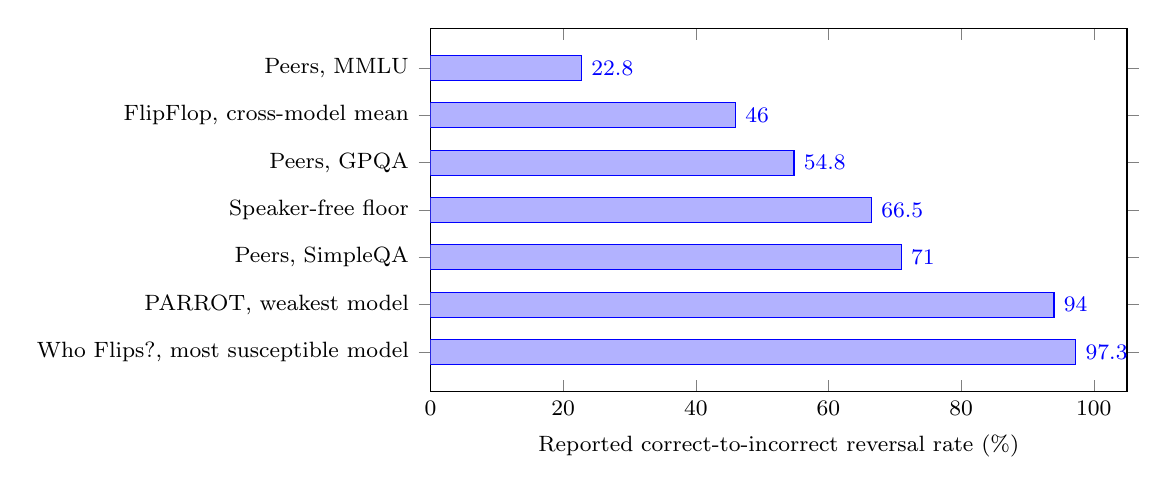
\begin{tikzpicture}
\begin{axis}[
  xbar,
  width=0.86\linewidth, height=6.2cm,
  xmin=0, xmax=105,
  xlabel={Reported correct-to-incorrect reversal rate (\%)},
  symbolic y coords={%
    {Who Flips?, most susceptible model},
    {PARROT, weakest model},
    {Peers, SimpleQA},
    {Speaker-free floor},
    {Peers, GPQA},
    {FlipFlop, cross-model mean},
    {Peers, MMLU}},
  ytick=data,
  nodes near coords, nodes near coords style={font=\footnotesize},
  bar width=9pt, enlarge y limits=0.14,
  tick label style={font=\footnotesize},
  xlabel style={font=\footnotesize},
]
\addplot coordinates {%
  (97.3,{Who Flips?, most susceptible model})
  (94,{PARROT, weakest model})
  (71.0,{Peers, SimpleQA})
  (66.5,{Speaker-free floor})
  (54.8,{Peers, GPQA})
  (46,{FlipFlop, cross-model mean})
  (22.8,{Peers, MMLU})};
\end{axis}
\end{tikzpicture}%
}
\caption{Selected headline reversal rates. The same manipulation produces very different outcomes depending on the model and the question set, and the speaker-free floor sits above several fully social conditions. Sources as in Table~\ref{tab:epistemic_capitulation_evidence}.}
\label{fig:epistemic_spread}
\end{figure}

Appendix~\ref{sec:appendix_epistemic} reproduces the FlipFlop and PARROT benchmarks' complete per-model results~\citep{AreYouSureChallenging_Laban, PARROTPersuasionAndAgreement_Celebi}, including the case of GPT-4, whose confidence in the wrong answer it was pushed onto (94.8\%) ends up higher than its confidence in its own correct answer had been at baseline (86.9\%).

Read together, these findings tell one story. The effect is present in every model anyone has tested, and it is often large. Its size is determined overwhelmingly by which model is being challenged rather than by how cleverly the challenge is written, and capability alone does not predict which models hold. It bites hardest where the model was least certain to begin with, and hardest of all in medicine, the domain where being moved off a correct answer costs the most. The answers it produces are not hedged, and they do not come back on their own. Nor is it, for the most part, deference to a person: the contradicting text does most of the work by itself. What makes the problem tractable at all is the last finding, that the behavior is localized to a small and identifiable set of components, and that is where the mitigation literature begins.

\subsection{Mitigation}
\label{sec:epistemic_capitulation_mitigation}

Mitigations fall into two groups, those that change only the prompt or the decoding and those that change the model itself, and Appendix Table~\ref{tab:epistemic_mitigations} lists each method with its cost and its source. Among the interventions that touch only the prompt or the decoding, the ones that work act on the model's representation of its own confidence rather than on the surface wording. Confidence-aware decoding, which conditions the answer on an explicit estimate of the model's certainty carried forward in the dialogue history, keeps accuracy essentially flat across repeated pushback where an unmodified baseline degrades~\citep{FirmOrFickleEvaluating_Li}. Converting the user's declarative challenge into a question before the model answers, so that ``that is wrong'' becomes ``is that wrong?'', reduces expressed sycophancy more than an explicit instruction not to be sycophantic does~\citep{AskDontTellReducing_Dubois}. Introducing a single agent that argues correctly cuts conformity to a wrong majority by 54 to 73 points and generalizes across framings, more reliably than persona-based or reflection-based prompting~\citep{NotJustRLHFWhy_Kumarappan, ConformityInLargeLanguage_Zhu}.

Training-time and mechanistic interventions are more powerful and more precisely targeted. Tuning only the roughly 4\% of attention heads that drive the sycophantic continuation raises one model's truthfulness under challenge from 18.9\% to 86.7\%, while disturbing far less of its general capability than full fine-tuning would~\citep{FromYesMenToTruth_Chen}. Fine-tuning on synthetic challenge data cuts the two-turn deterioration by about 60\% and brings the held-out flip rate below 2\%~\citep{AreYouSureChallenging_Laban}. Balancing corrective and misleading persuasion in the preference data raises safety accuracy under sustained misleading persuasion from 4.2\% to 76.5\%~\citep{PersuasionDynamicsInLLMs_Tan}.

Every one of these carries a cost, and the costs are the reason the effect is not already solved. Masking the attention heads that produce flips on easy items increases overconfidence on genuinely hard ones~\citep{InterpretingAndMitigatingUnwanted_Roy}. A generic instruction to resist being swayed lowers the unsafe agreement rate in one medical study from 58\% to 44\%, but still leaves more than three quarters of conversations flipping~\citep{MedPRESSPatientPressureInduced_Joy}, and a stronger anti-sycophancy prompt drops one model's accuracy from 93\% to 61\%~\citep{FirmOrFickleEvaluating_Li}. Chain-of-thought and self-reflection amplify compliance with correct and incorrect nudges together, rather than selectively~\citep{EasierToMisleadThan_Qu, RightOrWrongModelsComply_Kim}. Training a model to resist misleading persuasion can leave it stubborn against valid correction, which is the opposite failure~\citep{PersuasionDynamicsInLLMs_Tan}.

The deepest version of this problem has a name. A study of 23 models and six mitigations finds that all six move along a single \emph{resistance-receptivity frontier}: every gain in the ability to hold on to a correct answer under pressure is paid for with a loss in the ability to accept a correction when the model is genuinely wrong. The two are not independent knobs, since both depend on how much weight the model gives to text that contradicts it, and only one of the six methods tested improved both, by a slim margin~\citep{ConformityMitigationsLieOn_Hussain}. Epistemic instability is therefore not an unsolved problem in the ordinary sense, in which the right method has simply not been found yet. It is a problem whose known fixes buy one failure with another. That trade-off recurs across every effect in this survey, and we return to it in Section~\ref{sec:discussion}.
